\documentclass[
	a4paper,
	oneside,
	BCOR = 10mm,
	DIV = 12,
	12pt,
	headings = normal,
]{scrartcl}

%%% Length calculations
\usepackage{calc}
%%%

%%% Support for color
\usepackage{xcolor}
\definecolor{lightblue}{HTML}{03A9F4}
\definecolor{red}{HTML}{F44336}
%%%

%%% Including graphics
\usepackage{graphicx}
%%%

%%% Font selection
\usepackage{fontspec}

\setromanfont{STIX Two Text}[
	SmallCapsFeatures = {LetterSpace = 8},
]

\setsansfont{IBM Plex Sans}[
	Scale = MatchUppercase,
]

\setmonofont{IBM Plex Mono}[
	Scale = MatchUppercase,
]
%%%

%%% Math typesetting
\usepackage{amsmath}

\usepackage{unicode-math}
\setmathfont{STIX Two Math}
%%%

%%% List settings
\usepackage{enumitem}
\setlist[enumerate]{
	label*      = {\arabic*.},
	leftmargin  = *,
	labelindent = \parindent,
	topsep      = 1\baselineskip,
	parsep      = 0\baselineskip,
	itemsep     = 1\baselineskip,
}

\setlist[itemize]{
	label*      = {—},
	leftmargin  = *,
	labelindent = \parindent,
	topsep      = 1\baselineskip,
	parsep      = 0\baselineskip,
	itemsep     = 1\baselineskip,
}

\setlist[description]{
	font        = {\rmfamily\upshape\bfseries},
	topsep      = 1\baselineskip,
	parsep      = 0\baselineskip,
	itemsep     = 0\baselineskip,
}

%%%

%%% Structural elements typesetting
\setkomafont{pagenumber}{\rmfamily}
\setkomafont{disposition}{\rmfamily\bfseries}

% Sectioning
\RedeclareSectionCommand[
	beforeskip = -1\baselineskip,
	afterskip  = 1\baselineskip,
	font       = {\normalsize\bfseries},
]{section}

\RedeclareSectionCommand[
	beforeskip = -1\baselineskip,
	afterskip  = 1\baselineskip,
	font       = {\normalsize\bfseries\itshape},
]{subsection}

\RedeclareSectionCommand[
	beforeskip = -1\baselineskip,
	afterskip  = 1\baselineskip,
	font       = {\normalsize\bfseries},
]{subsubsection}

\RedeclareSectionCommand[
	beforeskip = -1\baselineskip,
	afterskip  = -0.5em,
	font       = {\normalsize\mdseries\scshape\addfontfeatures{Letters = {UppercaseSmallCaps}}},
]{paragraph}
%%%

%%% Typographic enhancements
\usepackage{microtype}
%%%

%%% Language-specific settings
\usepackage{polyglossia}
\setmainlanguage{ukrainian}
\setotherlanguages{english}
%%%

%%% Captions
\usepackage{caption}
\usepackage{subcaption}

%\DeclareCaptionLabelFormat{closing}{#2)}
%\captionsetup[subtable]{labelformat = closing}

%\captionsetup[subfigure]{labelformat = closing}

\captionsetup[table]{
	aboveskip = 0\baselineskip,
	belowskip = 0\baselineskip,
}

\captionsetup[figure]{
	aboveskip = 1\baselineskip,
	belowskip = 0\baselineskip,
}

\captionsetup[subfigure]{
	labelformat = simple,
	labelformat = brace,
}
%%%

%%% Table typesetting
\usepackage{booktabs}
\usepackage{longtable}

\usepackage{multirow}

\usepackage{array}
\newcolumntype{v}[1]{>{\raggedright\arraybackslash\hspace{0pt}}p{#1}}
\newcolumntype{b}[1]{>{\centering\arraybackslash\hspace{0pt}}p{#1}}
\newcolumntype{n}[1]{>{\raggedleft\arraybackslash\hspace{0pt}}p{#1}}
%%%

%%% Drawing with TikZ
% \usepackage{tikz}
% \usepackage{tikzscale}
% \usetikzlibrary{
% 	arrows.meta, % Stealth arrow tips
% 	positioning,
% 	shapes,
% 	trees,
% }

% \tikzset{> = stealth}
%%%

%%% Links and hyperreferences
\usepackage{hyperref}
\hypersetup{
	bookmarksnumbered = true,
	colorlinks      = false,
	linkbordercolor = red,
	urlbordercolor  = lightblue,
	pdfborderstyle  = {/S/U/W 1.5},
}
%%%

%%% Length adjustments
% Set baselineskip, default is 14.5 pt
\linespread{1.068966} % ~15.5 pt
\setlength{\emergencystretch}{1em}
\setlength{\parindent}{1.5em}
\newlength{\gridunitwidth}
\setlength{\gridunitwidth}{\textwidth / 12}
%%%

%%% Custom commands
\newcommand{\allcaps}[1]{{\addfontfeatures{LetterSpace = 8, Kerning = Off}#1}}
%%%

\begin{document}
% Клокун.
% 1 (О — 10). Поясніть поняття програмна бібліотека та різницю між динамічними і статичними бібліотеками. 
	\section{Поясніть поняття програмна бібліотека та~різницю між~динамічними і~статичними бібліотеками} 
		Програмна бібліотека~— це набір реалізацій поведінки, написаних в~рамках певної мови, який має чітко визначений інтерфейс для~виклику цієї поведінки. Інакше кажучи, це~програмний засіб, що~містить реалізацію заданих функцій, доступних за~чітко визначеним інтерфейсом, для~їх подальшого використання.

		Різниця між динамічними і~статичними бібліотеками полягає у~тому, що~зв'\-яз\-ки цільового виконуваного файлу з~функціями статичних бібліотек встановлюються у~момент компіляції, а~динамічних~— у~момент завантаження ресурсів або~виконання програми.

	%2 (К — 7). Поясніть поняття «драйвер-фільтр». Для чого можуть бути потрібні такі драйвери?} 
	\section{Поясніть поняття «драйвер-фільтр». Для чого можуть бути потрібні такі драйвери?} 
		% (Взято з MSDN, https://docs.microsoft.com/en-us/windows-hardware/drivers/kernel/filter-drivers)
		% Драйвер-фільтр~— це необов'язковий, опціональний драйвер, який розширює або модифікує поведінку пристрою. Драйвер-фільтр може обслуговувати один або декілька пристроїв.
		Драйвер-фільтр~— це необов'язковий, опціональний драйвер, який розширює або модифікує існуючу поведінку пристрою. Такі драйвери можуть знадобитись для розширення базового функціоналу, наприклад, управління живленням, прискорення пересування курсора мишою за допомогою відповідних трансформацій вхідних даних, впровадження додаткових перевірок безпеки вводу з клавіатури тощо. Драйвер-фільтр може обслуговувати один або декілька пристроїв.

		Існує декілька типів таких драйверів: драйвери-фільтри шин, драйвери-фільтри нижчого рівня та драйвери фільтри вищого рівня. Останні два типи також поділяються на пристроеві та класові: для одного певного пристрою або цілого класу пристроїв відповідно.

		Драйвери-фільтри шин зазвичай розширюють можливості шини та постачаються Microsoft або розробником пристрою. Такі драйвери можуть, наприклад, додавати пропрієтарні розширення та покращення до стандартного апаратного забезпечення шини.

		Для пристроїв, що описуються ACPI BIOS, менеджер живлення вбудовує ACPI-фільтр (драйвер-фільтр шини) над драйвером шини для кожного пристрою. Такий ACPI-фільтр наглядає за політикою живлення пристрою та вмикає або вимикає їх. Такий ACPI-фільтр прозорий і видимий іншим драйверами і відсутній на машинах без підтримки ACPI.

		Драйвери-фільтри нижчого рівня зазвичай змінюють поведінку апаратного забезпечення пристрою. Вони зазвичай необов'язкові, опціональні і надаються незалежними виробниками (вендорами) апаратного забезпечення. Для кожного пристрою можуть існувати і використовуватись будь-яка кількість драйверів-фільтрів нижчого рівня.

		Пристроевий драйвер-фільтр нижчого рівня (lower-level device filter driver) відстежує та/або модифікує запити вводу-виводи для певного пристрою. Зазвичай, такі фільтри перевизначають апаратну поведінку під очікувану специфікацію.

		Класовий драйвер-фільтр нижчого рівня відстежує та/або модифікує запити вводу-виводу для класу пристроїв. Наприклад, класовий драйвер-фільтр для пристроїв типу «миша» може реалізовувати прискорення за допомогою нелінійного перетворення даних про переміщення миші.

		Драйвери-фільтри вищого рівня зазвичай надають подальші розширення функціоналу для певного пристрою. Такі драйвери зазвичай створюються незалежними вендорами апаратного забезпечення та є необов'язковими. Для певного пристрою може бути необмежена кількість драйверів-фільтрів вищого рівня.

		\begin{figure}[!htbp]
			\centering
			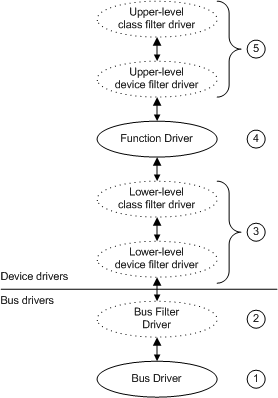
\includegraphics[height = 10\baselineskip]{./assets/y03s01-syssoft-mod-01-klokun-02-01.png}
			\caption{Рівні драйверів}
			\label{fig:02-01-driver-levels}
		\end{figure}

	% 3 (К — 7). Охарактеризуйте вкладки Properties (Властивості) та Events (Події) Інспектора Об'єктів інтегрованого середовища візуальної розробки (CBuilder/RAD Studio etc).
	\section{Охарактеризуйте вкладки \textenglish{Properties} (Властивості) та~\textenglish{Events} (Події) Інспектора Об'єктів інтегрованого середовища візуальної розробки (\textenglish{CBuilder/RAD Studio etc})}
		Вкладка \textenglish{Properties} Інспектора об'єктів дає змогу користувачу задавати властивості компонентів на формі під час проектування. Ця вкладка показує властивості вибраного на формі компонента і містить дві колонки: \textenglish{Property Name}~— назву властивості і \textenglish{Property Value}~— значення властивості. Редагування властивостей здійснюється за допомогою зміни необхідних значень властивостей. Сортування властивостей, перелічених у вкладці, можна виконувати як за алфавітним порядком, так і за категоріями.

		Вкладка \textenglish{Events} містить усі події для обраного компонента і форми. Ця вкладка містить дві колонки: \textenglish{Event Name}~— назву події і \textenglish{Event Handler}~— обробник події. Обробник події визначає, як компонент або форма реагує на певну подію. Щоб автоматично згенерувати декларацію обробника події, необхідно натиснути на праву колонку \textenglish{Event Handler} навпроти бажаної події.

	% 4 (Л — 7). Label, Panel.
	% 4.1 Охарактеризуйте компоненти інтегрованих середовищ візуальної розробки CBuilder RAD Studio.
	% 4.2 Розгляньте основні події цих компонентів.
	% 4.3 Вкажіть компоненти, які є аналогами розглянутих в середовищі Visual Studio. Для кожної пари компонентів розгляньте їх спільні риси і відмінності.
	% 4.4 Для розв'язання яких задач, на Ваш погляд, доцільно використовувати ці компоненти? (Дайте загальну відповідь та наведіть приклад програми, в якій доцільно використати компонент.)
	\section{\textenglish{Label, Panel}}
		\subsection{Охарактеризуйте компоненти \textenglish{Label, Panel} інтегрованих середовищ візуальної розробки \textenglish{CBuilder RAD Studio}}
			\textenglish{Label}~— це компонент, який виводить (додає) текст, що не може бути змінений користувачем на формі.

			\textenglish{Panel}~— це компонент, який створює пусту панель на формі, на якій можна розмістити інші компоненти. 

		\subsection{Розгляньте основні події цих компонентів}
			Основні події компонента \textenglish{Label} виконують зазначені дії у таких випадках:
			\begin{enumerate}[noitemsep]
				\item \textenglish{OnClick}~— при~одноразовому натисканні на~компонент.
				\item \textenglish{OnDblClick}~— при~подвійному натисканні на~компонент.
				\item \textenglish{OnDragDrop}~— при~перетягуванні об'єкту в~області компонента.
				\item \textenglish{OnDragDrop}~— при~відпущенні перетягуваного об'єкту в~області компонента.
				\item \textenglish{OnContextPopup}~— при~виклику вспливаючого меню за~допомогою правої клавіші миші або~з~клавіатури.
				\item \textenglish{OnMouseActivate}~— при~натисканні клавіші миші, коли курсор вказує на~компонент і~материнська форма неактивна.
				\item \textenglish{OnMouseDown}~— при~натисканні клавіші миші, коли курсор вказує на~компонент.
				\item \textenglish{OnMouseUp}~— при~натисканні клавіші миші, коли курсор вказує на~компонент.
				\item \textenglish{OnMouseEnter}~— при~наведенні курсору в~область компонента.
				\item \textenglish{OnMouseLeave}~— при~виведенні курсору з~області компонента.
				\item \textenglish{OnMouseMove}~— при~пересуванні курсору в~області компонента.
			\end{enumerate}

			Для компонента \textenglish{Panel} характерні основні події компонента~\textenglish{Label}, доповнені такими подіями, що виконують задані дії у таких випадках:
			\begin{enumerate}[noitemsep]
				\item \textenglish{OnCanResize} — при спробі змінити розмір компонента.
				\item \textenglish{OnEnter} — при отриманні компонентом фокусу.
				\item \textenglish{OnExit} — при переході фокусу від одного компонента до іншого.
				\item \textenglish{OnResize} — при закінченні зміни розміру компонента.
				\item \textenglish{OnUndock} — при відкріпленні (\textenglish{undock}) компонента.
			\end{enumerate}

		\subsection{Вкажіть компоненти, які є аналогами розглянутих в середовищі \textenglish{Visual Studio}. Для кожної пари компонентів розгляньте їх спільні риси і відмінності.}
			В середовищі \textenglish{Visual Studio} аналогічні компоненти мають назви \textenglish{Label, Panel} відповідно. Оскільки ці компоненти є базовими для створення програм, за основним функціоналом вони ідентичні: \textenglish{Label} відображає текст та дозволяє змінювати його розмір, шрифт, колір, а також інші елементи представлення в обох середовищах; \textenglish{Panel} дозволяє вміщувати інструменти в обох середовищах, може підтримувати зміну розміру, відкріплення тощо.
			
			До відмінностей компонентів відносяться наявність та назви властивостей: \textenglish{Visual Studio} дозволяє налаштувати більшу кількість властивостей порівняно з \textenglish{C++ Builder}. Наприклад, підтримку засобів для людей з обмеженими можливостями: відповідні параметри \textenglish{AccessibleDescription, AccessibleName, AccessibleRole} наявні лише у~\textenglish{Visual Studio}. Наступною відмінністю є кількість і назви подій, пов'язаних з компонентами: \textenglish{Visual Studio} знову надає більшу кількість обробників подій, і майже кожна назва змінюється, а в рамках даної модульної контрольної роботи наводити порівняльний список назв не несе користі і не має сенсу. 

		\subsection{Для розв'язання яких задач, на Ваш погляд, доцільно використовувати ці компоненти? (Дайте загальну відповідь та наведіть приклад програми, в якій доцільно використати компонент)}
			 Компонент \textenglish{Label} зазвичай використовується щоб назвати та відмітити для користувача інший компонент на формі. Наприклад, його доцільно використати для позначення полів вводу та результату у програмі, що вираховує швидкість за пройденим шляхом та часом.

				Як правило, компонент \textenglish{Panel} використовується для створення панелі інструментів у програмі. Цей компонент доцільно застосувати у графічному редакторі для групування різноманітних інструментів малювання та редагування зображення.

\end{document}



Ульчич.
1 (Ь — 15). Охарактеризуйте призначення драйверів та служб в комп'ютерній системі. Наведіть приклади драйверів та служб.

2 (Ч — 15). Розгляньте дії, які необхідно виконати, щоб розробити у візуальному середовищі розробки програму, яка має головне меню.

3 (У — 14). Поясніть значення понять «форма» та «проект» у візуальному середовищі розробки. Які можливості надає розробнику використання проектів та форм?

4 (Л — 7). Label, Panel.
